\chapter{Método Proposto}



% -.~.-.~.-.~.-.~.-.~.-.~.-.~.-.~.-.~.-.~.-.~.-
\section{Visão geral}

O método proposto divide-se nas seguintes etapas:

\missingfigure[figheight=100mm]{Diagrama do método}


% -.~.-.~.-.~.-.~.-.~.-.~.-.~.-.~.-.~.-.~.-.~.-
\section{Modelo do robô}

Nesta seção, são detalhados os procedimentos para representar o manipulador
robótico como um conjunto MBS e utilizá-lo para simular as trajetórias
referentes a uma determinada tarefa. O manipulador será descrito pelo conjunto
de Sistemas de Coordenadas (SC's) referente a cada uma de suas juntas, pelas
distâncias entre os SC's e posição dos centros de massa de cada elo, e pelos
parâmetros de massa e momento de inércia de cada elo. Os elos do robô e a
ferramenta acoplada no efetuador representam cada corpo do sistema MBS. A
modelagem do manipulador é simplificada utilizando as rotinas de CAS
desenvolvida especialmente para MBS, o Sophia, assim como a notação algébrica de
Lesser, apresentada na seção~\ref{sec::sophia-kane}.

\subsection{Descrição do braço robótico} \label{sec::descricao_mh12}

O manipulador escolhido para estudo é o mesmo que será utilizado no projeto EMMA
para revestimento de superfícies metálicas por HVOF. Trata-se de um robô
comercial modelo MH12, da série MOTOMAN, fabricado pela Yaskawa Motoman
(Figura~\ref{fig::mh12_foto}).

\begin{figure}[h]
    \centering
    \begin{subfigure}[b]{0.3\textwidth}
        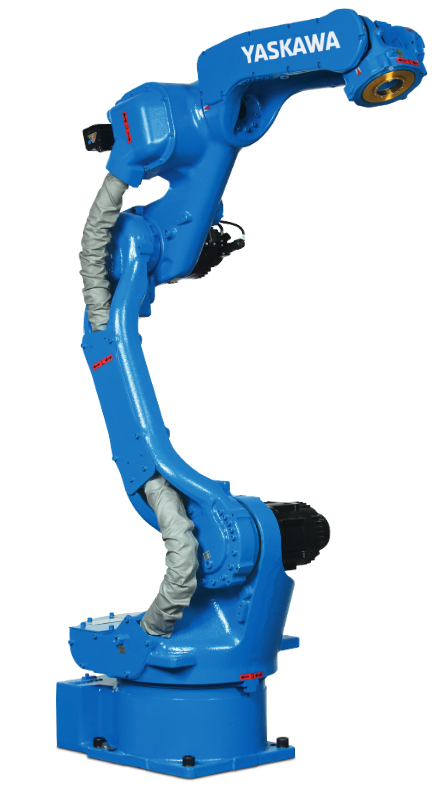
\includegraphics[width=\textwidth]{figs/mh12_foto}
        \caption{MOTOMAN MH12. \\Fonte: adaptada de}
        \label{fig::mh12_foto}
    \end{subfigure}
    \quad %add desired spacing between images, e. g. ~, \quad, \qquad, \hfill
    % etc.
      %(or a blank line to force the subfigure onto a new line)
    \begin{subfigure}[b]{0.5\textwidth}
        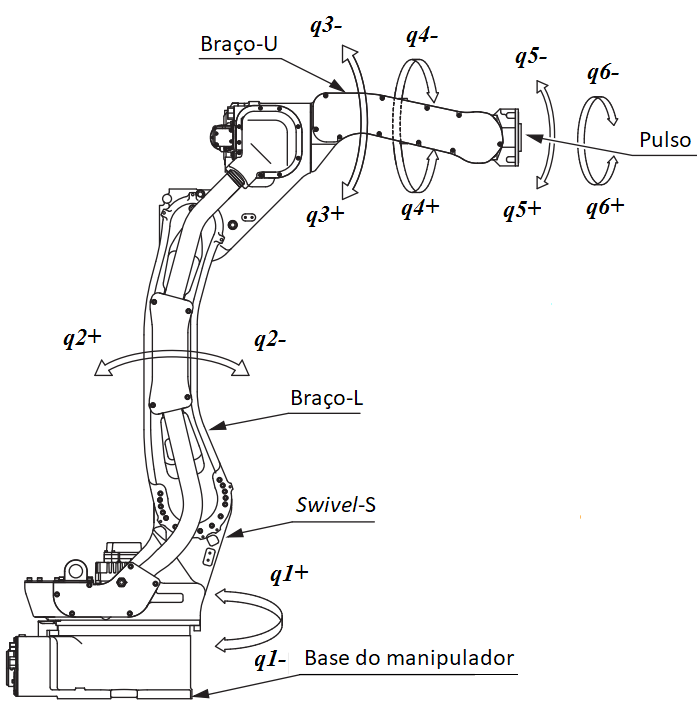
\includegraphics[width=\textwidth]{figs/mh12_diagram}
        \caption{Diagrama dos elos e juntas. \\Fonte: adaptada de}
        \label{fig::mh12_diagram}
    \end{subfigure}
    \caption{Manipulador robótico para modelo}\label{fig::resumo_mh12}
    \todo[inline]{Inncluir referências das figuras - MH12 specsheet}
\end{figure}

\begin{table}[h]
\centering
\caption{Sistemas de coordenadas, elos e coordenadas generalizadas}
\label{tab::resumo_mh12}
\begin{tabular}{@{}clc@{}}
\toprule
SC & Elo              & \multicolumn{1}{l}{Coord. gen. associada} \\ \midrule
Z  & Pedestal do robô & -                                         \\
S  & \textit{Swivel}  & q1                                        \\
L  & Braço inferior   & q2                                        \\
U  & Braço superior   & q3                                        \\
R  & Braço de rolagem & q4                                        \\
B  & Pulso            & q5                                        \\
T  & Efetuador        & q6                                        \\ \bottomrule
\end{tabular}
\end{table}

Este robô é um braço antropomórfico de 6 juntas rotacionais e portanto 6 graus
de liberdade (6 gdl), contendo o último elo um porta-ferramentas que suporta uma
carga útil de até 12 kg. A Figura~\ref{fig::mh12_diagram} apresenta os nomes dos
elos e coordenadas generalizadas associados a cada um dos sistemas de
coordenadas e são resumidos na Tabela~\ref{tab::resumo_mh12}.

O alcance horizontal deste manipulador chega a 1,440~m, e vertical a
2,511~m. Estão representados no diagrama do espaço de trabalho na
Figura~\ref{fig::workspace} em que a área sombreada é formada por todos os
pontos alcançáveis pelo manipulador, dentro dos limites de cada junta.

\begin{figure}[h]
	\centering 
 	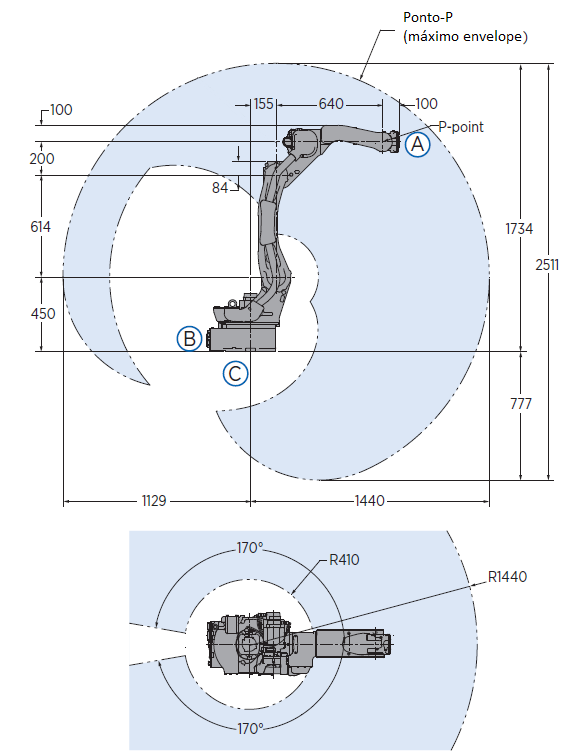
\includegraphics[width=0.7\textwidth]{figs/workspace}
 	\caption[Vistas lateral e superior do espaço de trabalho]{Vistas lateral e
 	superior do espaço de trabalho. \\Fonte: adaptada de}
 		\todo[inline]{Inncluir referência da figura - MH12 specsheet}
 	\label{fig::workspace}
\end{figure}

Conforme discutido na seção~\ref{sec::manind}, este tipo de braço robótico
permite desacoplar o sistema em 2 problemas: posicionamento e orientação. Logo,
para simplificar o modelo e o cálculo da cinemática inversa, serão consideradas
as 3 primeiras juntas para posicionamento e 3 últimas (pulso esférico) para
orientação da ferramenta.

A última junta, no efetuador, tem a finalidade de orientar a ferramenta em torno
do seu eixo axial. Como o processo de revestimento por HVOF independe desta
orientação, esta junta não será incluída, mantendo este acoplamento rígido, o
que transforma os dois últimos elos em apenas um corpo.
Como resultado, tem-se um sistema de 5 gdl.


\subsection{Cinemática Direta}

Como foi discutido na seção~\ref{sec::cinematica}, o procedimento mais utilizado
para a modelagem cinemática de manipuladores robóticos é o método dos parâmetros
de Denavit-Hartenberg (parâmetros D-H). Apesar de sua popularidade e vasta
utilização na modelagem cinemética de manipuladores variados, este método possui
regras que acabam restringindo uma livre escolha dos sistemas de coordenadas e
as direções dos eixos de referência. Dependendo da geometria do robô, pode ser
uma tarefa trabalhosa definir os parâmetros e referenciais mais convenientes, e
que resultem em um sistema final simplificado.

Um maior controle sobre a escolha dos referenciais e dos parâmetros da geometria
pode reduzir significativamente o custo computacional do modelo.
Neste sentido, o Sophia-Maple é uma ferramenta mais flexível, que permite, ao
usuário, total liberdade sobre a escolha dos referenciais, sem nenhum aumento de
complexidade. Uma escolha estratégica da posição e orientação dos sistemas de
coordenadas pode resultar em equações cinemáticas e transformações de
referenciais mais simplificadas. Neste trabalho serão utilizadads as rotinas do
Sophia para modelagem da cinemática direta do manipulador robótico.

\subsubsection{Sistemas de Coordenadas e Transformações Homogêneas}

A primeira etapa para obter-se as equações cinemáticas será definir o sistema de
coordenadas fixo em cada elo do robô. A Figura~\ref{fig::scs} é um modelo CAD do
manipulador e apresenta a posição de cada SC, na configuração inicial.

\begin{figure}[h]
    \centering
    \begin{subfigure}[b]{0.20\textwidth}
        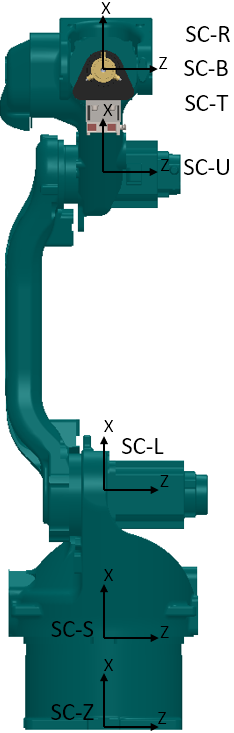
\includegraphics[width=\textwidth]{figs/sc_front}
        \caption{Vista frontal}
        \label{fig::sc_front}
    \end{subfigure}
    \quad %add desired spacing between images, e. g. ~, \quad, \qquad, \hfill
    % etc.
      %(or a blank line to force the subfigure onto a new line)
    \begin{subfigure}[b]{0.7\textwidth}
        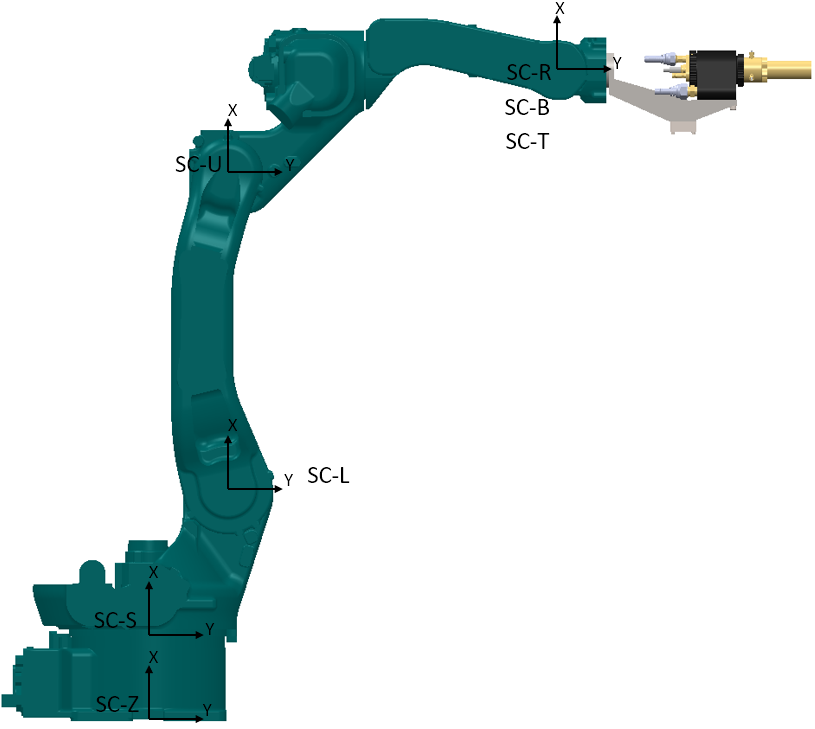
\includegraphics[width=\textwidth]{figs/sc_lat}
        \caption{Vista lateral}
        \label{fig::sc_lat}
    \end{subfigure}
    \caption{Sistemas de coordenadas do robô}\label{fig::scs}
\end{figure}

Na vista frontal (Figura~\ref{fig::sc_front}) nota-se que foi escolhida uma
configuração em que todos os SC's estivessem no mesmo plano XY. Outra observação
é que os SC's R, B e T estão fixados no mesmo ponto. que representa a origem do
``pulso'' do braço robótico. Estas considerações reduzem a quantidade de termos
das equações cinemáticas. Também terão grande impacto no cálculo da cinemática
inversa, como será visto na seção~\ref{sec::ikin_mh12}.

Logo, pode-se escrever as relações entre estes referenciais em termos das
coordenadas generalizadas do sistema, para obter as transformações entre cada
SC. No Sophia-Maple isto é feito com o uso da função \textit{chainSimpRot}, da
seguinte forma:

\medskip \noindent {\tt > chainSimpRot( [Z,S,1,q1], [S,L,3,q2], [L,U,3,q3],
[U,R,2,q4], [R,B,3,q5], [B,T,2,q6] )} \medskip 

Esta função cria as matrizes de rotação entre os referenciais do sistema,
informando a cada transformação, o eixo de rotação
(onde 1=X, 2=Y e 3=Z) e a coordenada generalizada associada
(q1,~\ldots~,q6). Foi utilizada a forma de coordenadas relativas entre cada SC.

Como exemplo, considere o termo {\tt [L,U,3,q3]}. Representa uma rotação de um
ângulo q3, do SC-U em relação ao SC-L, em torno do eixo Z.
Logo, a matriz Transformação Homogênea entre o referencial inercial Z e o braço
superior U seria:
%
$$ R_{Z}^{U} = R_{Z}^{S} R_{S}^{L} R_{L}^{U} $$
%
A função \textit{Rmx} do Sophia-Maple retorna a matriz de rotação entre quaisquer
sistemas de coordenadas. No Sophia-Maple, escreve-se:

\medskip \noindent {\tt > Rmx(Z,U)} \medskip 

E obtém-se o resultado:
%
$$ R_{Z}^{U} = \left( \begin {array}{ccc} {\it c2}\,{\it c3}-{\it s2}\,{\it
s3}&-{ \it c2}\,{\it s3}-{\it s2}\,{\it c3}&0\\ \noalign{\medskip}{\it c1}\,{
\it c2}\,{\it s3}+{\it c1}\,{\it s2}\,{\it c3}&{\it c1}\,{\it c2}\,{
\it c3}-{\it c1}\,{\it s2}\,{\it s3}&-{\it s1}\\ \noalign{\medskip}{
\it s1}\,{\it c2}\,{\it s3}+{\it s1}\,{\it s2}\,{\it c3}&{\it s1}\,{
\it c2}\,{\it c3}-{\it s1}\,{\it s2}\,{\it s3}&{\it c1}\end {array}
 \right) $$
 %
 A matriz acima foi escrita em notação trigonométrica simplificada, em que c1,
 s1, ,c2, s2, \ldots, e assim por diante, representam as funções senos e
 cossenos dos ângulos das coordenadas generalizadas q1, \ldots, q5. Para melhor
 visualização das matrizes e equações, esta notação será utilizada em todo o
 trabalho.
 
\subsubsection{Vetores posição e centros de massa}

A segunda etapa é definir os vetores posição dos centros de massa de cada corpo.
Para isso, define-se auxiliarmente os vetores posição entre cada SC, desde o
referencial inercial Z até o efetuador em T. Será utilizada a notação de Lesser,
por meio dos \textit{Evectors}, como descrito na seção~\ref{sec::sophia-kane}
para representar esses vetores.

Logo, de maneira geral, pode-se escrever a posição de qualquer ponto pela
seguinte relação:
%
\begin{align}
	^{Z}\mathbf{p}^{k} = ^{Z}\mathbf{p}^{k-1} + ^{k-1}\mathbf{p}^{k} \\
	^{Z}\mathbf{pcm}^{k} = ^{Z}\mathbf{pcm}^{k-1} + ^{k}\mathbf{pcm}
	\label{eq::pcm}
\end{align}
%
Onde $^{Z}\mathbf{p}^{k}$ é o vetor posição do referencial $k$ em relação ao
referencial inercial $Z$ e analogamente $^{Z}\mathbf{pcm}^{k}$ é o vetor
posição do centro de massa do corpo $k$, tal que $k$ varia em \{S,L,U,B,T\},
sistemas de coordenadas do robô.
No Sophia-Maple escreve-se:

\medskip \noindent {\tt > pZ:= Evector(0,0,0,Z)} \\
\noindent {\tt > for k from corpo[1] to corpo[6] do \\
\indent p||k:= p||{k-1} \&++ Evector(p||{k-1}||{k}||x, p||{k-1}||{k}||y,
\indent p||{k-1}||{k}||z, k-1) \\
end do:} \medskip 

E para os centros de massa:

\medskip \noindent {\tt > for k from corpo[1] to corpo[6] do \\
\indent pcm||k:= p||{k} \&++ Evector(pcm||{k}||x, pcm||{k}||y, pcm||{k}||z, k)
\\ end do:} \medskip 

\todo[inline]{Incluir figura com vetores posição e centros de massa}

\subsubsection{Velocidades}

As velocidades dos centros de massa de cada corpo são calculadas como a derivada
do vetor posição com respeito ao referencial inercial. Logo, a derivada da
equação~\ref{eq::pcm} em Z:
%
\begin{equation}
	\mathbf{V}^{k} = \frac{^{Z}\mathrm{d} }{\mathrm{d} t}
	\mathbf{pcm}^{k} \label{eq::veloc}
\end{equation}
%
O Sophia-Maple possui um poderoso conjunto de rotinas para diferenciação dos
\textit{Evectors} com relação ao referencial inercial, por meio da função
\textit{cdft}, que reconhece automaticamente o referencial em que cada vetor
está descrito e realiza o cálculo diferencial vetorial. Logo, pode-se escrever o
seguinte comando para definir as velocidades de acordo com a
equação~\ref{eq::veloc}:

\medskip \noindent {\tt > for k from corpo[1] to corpo[6] do \\
\indent v||k:= cdft(pcm||{k}, Z) \\
end do:} \medskip 

As velocidades angulares serão a taxa de variação angular das matrizes de
rotação entre os referenciais. Serão definidas as velocidades angulares de cada
corpo em relação ao referencial inercial. Conforme apresentado na
seção~\ref{sec::cinematica} pode-se escrever a velocidade angular de uma matriz
rotação $R(t)$ como:
%
\begin{equation}
	\frac{\mathrm{d} R}{\mathrm{d} t} = S \cdot R(t)
\end{equation}
%
Onde $S$ é o tensor velocidade angular associado a $\omega$.
%
\begin{align}
% eq1
& S = \begin{pmatrix}
0				& -\omega_{z}(t)	& \omega_{y}(t) \\ 
\omega_{z}(t)	& 0					& -\omega_{x}(t) \\ 
-\omega_{y}(t)	& \omega_{x}(t)		& 0
\end{pmatrix} \\
% eq2
& \omega = [\omega_{x}, \omega_{y}, \omega_{z}]^{T}
\end{align}
%
No Sophia-Maple o tensor $S$ pode ser calculado através da função
\&\textit{VtoD}. Por exemplo, o tensor entre os referenciais SC-L e SC-S seria:
%
$$
S_{L}^{Z} = \left( \begin {array}{ccc} 0&-{\it q2t}&-\sin \left( {\it q2}
 \right) {\it q1t}\\ \noalign{\medskip}{\it q2t}&0&-\cos \left( {\it 
q2} \right) {\it q1t}\\ \noalign{\medskip}\sin \left( {\it q2}
 \right) {\it q1t}&\cos \left( {\it q2} \right) {\it q1t}&0
\end {array} \right)
$$
%
Porém, pode-se ainda fazer o uso da função \textit{aV} que
calcula diretamente o vetor velocidade angular $^{A}\omega^{B}$ entre dois
referenciais. O que retornaria o seguinte vetor:
%
$$
^{Z}\omega^{L} = [-{\it q1t},\sin \left( {\it q1} \right) {\it q2t},-\cos
\left( {\it q1} \right) {\it q2t}]
$$
%
No caso do manipulador, são calculadas as velocidades de cada corpo em relação
ao referencial Z. São definidos da seguinte forma:

\medskip \noindent {\tt > for k from corpo[1] to corpo[6] do \\
\indent w||k:= aV(Z, corpo[k]) \\
end do:} \medskip 

Podemos finalmente escrever o vetor Velocidades Generalizadas, que nada mais é
que um \textit{Kvector} que fornece a lista de \textit{Evectors} referente às
velocidades lineares e angulares calculadas. Logo, o vetor velocidades
generalizadas tem a seguinte forma:
%
\begin{equation}
	v_{k} = [ v_{1},\ldots, v_{n}, \omega_{1},\ldots, \omega_{n}, 2n ]
\end{equation}
%
Onde cada termo do \textit{Kvector} é um \textit{Evector} da velocidade
generalizada.
Por fim, o último termo representa a quantidade de \textit{Evectors} que formam o
\textit{Kvector}.

\subsubsection{Hiperplano tangente}

Uma vez que as velocidades generalizadas foram definidas pode-se obter o
conjunto de vetores tangentes, pelo cálculo das velocidades parciais, que formam
o chamado hiperplano tangente.
Este plano é uma generalização da superfície que restringe o movimento do
sistema multicorpo e é obtido pela diferenciação das velocidades com respeito
às coordenadas generalizadas, conforme visto na seção~\ref{sec::cinematica}. As
velocidades parciais são calculadas pela expressão das velocidades
generalizadas, na equação~\ref{eq::velgen}. O termo explicitado na
equação~\ref{eq::tau} define o vetor tangente associado a i-ésima coordenada
generalizada.
%
\begin{gather}
%eq1
	^{R}\mathbf{v} = \frac{\mathrm{d} \mathbf{r}}{\mathrm{d} t} = \sum_{i}^{n}
	\dot{q_{i}} \frac{\partial r}{\partial q_{i}} + \frac{\mathrm{d}
	q_{i}}{\mathrm{d} t} \label{eq::velgen}\\
%eq2
	\dot{q_{i}} \frac{\partial r}{\partial q_{i}} = \tau_{i} \label{eq::tau}
\end{gather}
%
A função \textit{KMtangents} do Sophia-Maple obtém os termos que formam os
vetores tangentes em \textit{Kvectors} para cada coordenada generalizada. O
conjunto que forma o hiperplano tangente introduz uma estrutura do Sophia, dos
super \textit{Kvectors}, ou \textit{SKVector}. Esta estrutura facilitará a
projeção das equações dinâmicas no hiperplano tangente. Logo, para o manipulador
escreve-se:

\medskip \noindent {\tt > tau:= KMtangents(vK,u,6):} \medskip 


\subsection{Dinâmica}

Definida a cinemática direta do manipulador, deseja-se obter as forças de
inércia e externas generalizadas que fornecerão as equações de movimento do
sistema. Nesta seção primeiramente são introduzidos os parâmetros de inércia de
cada corpo do manipulador e como foram obtidos.

\subsubsection{Parâmetros de inércia do manipulador robótico}

Os parâmetros de inércia são a massa e o momento de inércia de cada corpo do
sistema. É importante notar que não é possível obter um modelo dinâmico preciso
apenas com as informações contidas nos manuais e fichas técnicas do manipulador
robótico. Infelizmente os parâmetros de inércia individuais de cada corpo não
são fornecidos pelos fabricantes e, portanto, serão estimados. 

Do manual do MOTOMAN MH12\todo{incluir ref: manual mh12}, tem-se que a massa
total do robô é de 130~kg. Também é disponibilizado, diretamente pelo
fabricante, um modelo CAD com ótimo detalhamento de cada corpo individualmente.

O programa SolidWorks foi utilizado para obter informações importantes para a
estimativa dos parâmetros de inércia. Nele é possível analisar cada elo em
separado e obter o seu volume. Com isso, pode-se obter uma massa específica
média do robô, de acordo com a equação~\ref{eq::rho}.
%
\begin{equation}
	\rho_{m} = M_{total}\sum_{corpo[1]}^{corpo[n]} V_{i} \label{eq::rho}
\end{equation}
%
Logo, pode-se estimar a massa de cada corpo, calculada pelo produto da massa
específica média $\rho_{m}$ e o volume, de acordo com a
equação~\ref{eq::massai}.
%
\begin{equation}
	m_{i} = \rho_{m} \cdot V_{i} \label{eq::massai}
\end{equation}
%
A massa da ferramenta acoplada ao efetuador foi obtida precisamente, pelo
projeto CAD do suporte, no SolidWorks, e informação do fabricante do dispositivo
HVOF.
A Tabela~\ref{tab::massa_mh12} apresenta os resultados da massa estimada em cada
corpo:
%
\begin{table}[h]
\centering
\caption{Resultado do cálculo da massa de cada corpo}
\label{tab::massa_mh12}
\begin{tabular}{@{}clc@{}}
\toprule
\textbf{Corpo}                      & \textbf{Volume} [$m^3$] & \multicolumn{1}{l}{\textbf{Massa} [kg]} \\ \midrule 
Z 									& 0,01595         & 40,5							   \\
S                                   & 0,01443         & 36,7                               \\
L                                   & 0,00579         & 14,7                               \\
U                                   & 0,00997         & 25,3                               \\
R                                   & 0,00399         & 10,1                               \\
B                                   & 0,00100         & 2,5                                \\
T                                   & 0,00005         & 0,13                               \\
Ferramenta                          & -		          & 5,97							   \\ \midrule
\textbf{Volume total}~$=$           & 0,05119        & \multicolumn{1}{c}{$m^3$}	       \\
\multicolumn{1}{r}{\textbf{$\rho_m =$}} & 2540          &
\multicolumn{1}{c}{$kg/{m^3}$}     \\ \bottomrule
\end{tabular}
\end{table}
%

Para este modelo dinâmico, não será utilizada a última junta do robô, como foi
explicado na seção~\ref{sec::descricao_mh12}, de forma que pode-se considerar os
corpos ``B, T e Ferramenta'' como um único corpo. Assim, as propriedades de
massa e momento de inércia podem ser somadas e condensadas em uma única
descrição. A partir deste ponto, estes 3 últimos corpos serão tratadaos como um
único corpo e será utilizada a denominação do corpo B para representar esse
conjunto, com seu sistema de referência fixado em SC-B.

O programa SolidWorks também foi utilizado para obter as posições do centro de
massa e momentos de inércia de cada elo.
Foi considerado que a massa calculada é distribuida homogeneamente no volume.
Isto resulta na posição estimada, fornecida pelo programa. A
Tabela~\ref{tab::resumo_cm} resume os valores encontrados para a posição do
centro de massa com respeito ao referencial de cada elo e a
Figura~\ref{fig::pcm_mh12} ilustra no modelo CAD a posição aproximada.
%
\begin{table}[h]
\centering
\caption{Posição do centro de massa}
\label{tab::resumo_cm}
\begin{tabular}{@{}cccc@{}}
\toprule
\textbf{Corpo} & \textbf{x [m]} & \textbf{y [m]} & \textbf{z [m]} \\ \midrule
Z              & 0,079      & -0,050     & 0,000      \\
S              & 0,124      & 0,027      & 0,008      \\
L              & 0,281      & -0,025     & -0,115     \\
U              & 0,123      & 0,115      & -0,025     \\
R              & 0,039      & -0,224     & 0,004      \\
B              & -0,011     & 0,146      & 0,000      \\ \bottomrule
\end{tabular}
\end{table}
%

\begin{figure}[h]
	\centering 
 	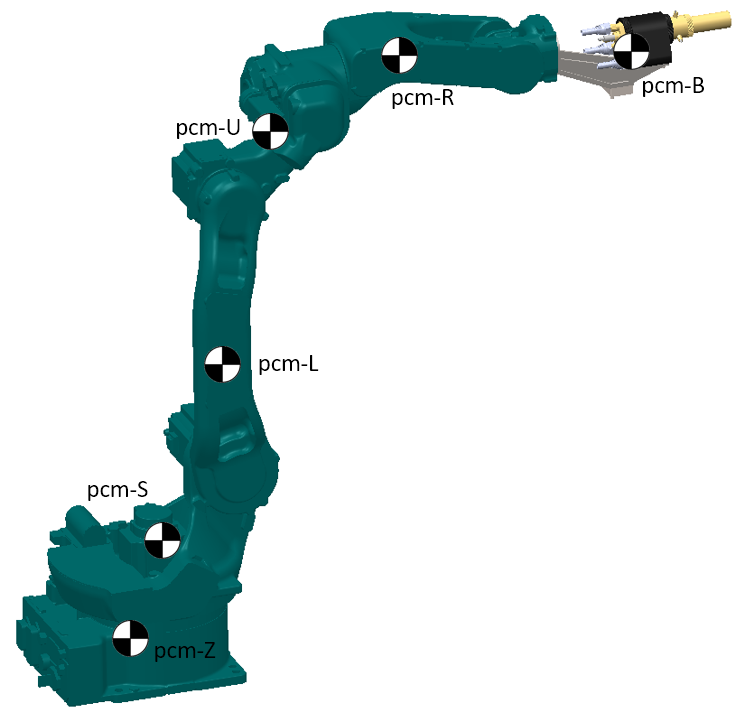
\includegraphics[width=0.7\textwidth]{figs/pcm_mh12}
 	\caption{Posição aproximada dos centros de massa}
 	\label{fig::pcm_mh12}
\end{figure}

Agora podem ser obtidos os momentos de inércia de cada elo obtidos no
centro de massa e alinhados ao sistema de coordenadas daquele elo. O programa
fornece esses valores, que são apresentados a seguir.
%
\begin{align*}
InZ &=& \left( \begin {array}{ccc}  0,811& 0,293& 0,091\\ \noalign{\medskip}
 0,293& 0,695& 0,064\\ \noalign{\medskip} 0,091& 0,064& 0,923
\end {array} \right) & \quad InS &=& \left( \begin {array}{ccc}  0,811& 0,293& 0,091\\ \noalign{\medskip}
 0,293& 0,695& 0,064\\ \noalign{\medskip} 0,091& 0,064& 0,923
\end {array} \right) \\
InL &=&  \left( \begin {array}{ccc}  0,051&-
0,008&- 0,032 \\ \noalign{\medskip}- 0,008& 0,791& 0,011\\ \noalign{\medskip}- 0,032
& 0,011& 0,798\end {array} \right) & \quad InU &=& \left( \begin {array}{ccc} 
0,314& 0,149&- 0,077\\ \noalign{\medskip} 0,149& 0,367&- 0,057\\ \noalign{\medskip}- 0,077&- 0,057& 0,418
\end {array} \right) \\
InR &=&  \left( \begin {array}{ccc}  0,173&-
0,014& 0,001\\ \noalign{\medskip} - 0,014& 0,052& 0,004\\ \noalign{\medskip} 0,001& 0,004& 0,148
\end {array} \right) & \quad InB &=&  \left( \begin {array}{ccc}  0,235&- 0,018& 0,0\\ \noalign{\medskip}-
 0,018& 0,039& 0,0\\ \noalign{\medskip} 0,0& 0,0& 0,243\end {array}
 \right)
\end{align*}
%
No Sophia-Maple estes tensores são construidos com a função
\textit{EinertiaDyad}, que aproveita o fato dos tensores de inércia serem
simétricos e recebe 6 argumentos para os termos da matriz e um para o sistema de
coordenadas de referência em que foi obtido o tensor. Define-se portanto cada
tensor da seguinte forma:

\medskip \noindent {\tt > for i from corpo[1] to corpo[6] do \\
\indent In||(corpo[i]):= EinertiaDyad( \\
\indent In||(corpo[i])||11, In||(corpo[i])||22, \\
\indent In||(corpo[i])||33, In||(corpo[i])||12, \\
\indent In||(corpo[i])||13, In||(corpo[i])||23, sc[i]) \\
end do:}




\subsection{Cinemática Inversa}\label{sec::ikin_mh12}

\subsection{Tarefa e trajetória}

\subsection{Modelo teórico MBS -- Robô}


% -.~.-.~.-.~.-.~.-.~.-.~.-.~.-.~.-.~.-.~.-.~.-
\section{Modelo da base}

\subsection{Geometria e CAD}

\subsection{Matriz de Rigidez}

\subsection{Matriz de Amortecimento}

\subsection{Análise Elementos Finitos}

\subsection{Modelo teórico MBS -- Base}


% -.~.-.~.-.~.-.~.-.~.-.~.-.~.-.~.-.~.-.~.-.~.-
\section{Ensaio Experimental}

\subsection{Bancada experimental}

\subsection{Programas de aquisição dos dados experimentais}

\subsection{Tratamento dos dados}

\subsection{Cálculo dos parâmetros modais da estrutura}


% -.~.-.~.-.~.-.~.-.~.-.~.-.~.-.~.-.~.-.~.-.~.-
\section{Modelo acoplado robô e base}

\subsection{Base rígida}

\subsection{Base flexível}


% -.~.-.~.-.~.-.~.-.~.-.~.-.~.-.~.-.~.-.~.-.~.-
\section{Estudos de casos para avaliação do método}

\subsection{Trajetórias do efetuador}

\subsection{Base rígida}

\subsection{Base de testes}

\subsection{Base modular PRP}

\subsection{Base com pouca rigidez}
